\section{Registrar Programa Sintético}
Para registrar un Programa Sintético correspondiente a una Unidad de Aprendizaje, primero se da click en en la pestaña \IUbutton{Ver Tareas} y la siguiente pantalla será desplegada:

\begin{figure}[H]
    \centering
    \hypertarget{RegLUA}{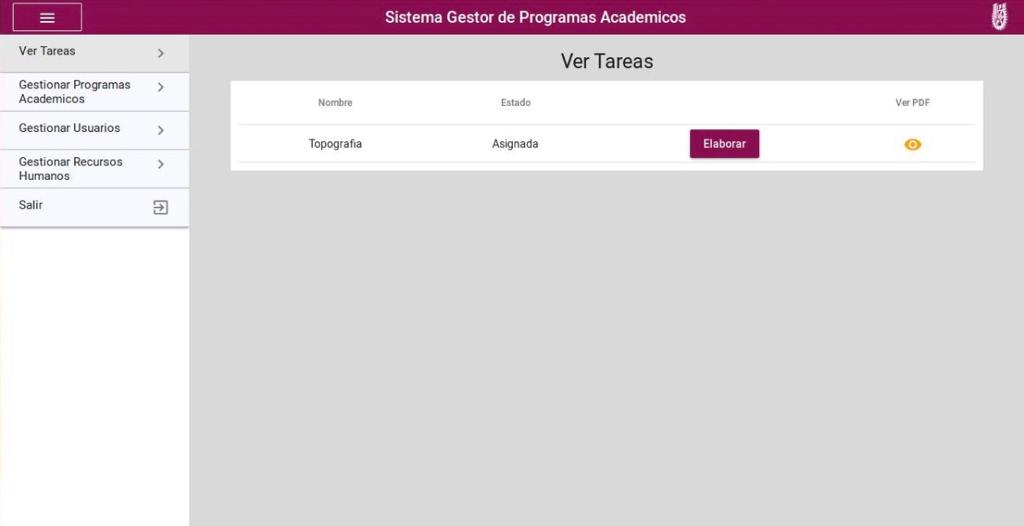
\includegraphics[width=0.7\linewidth]{images/SP6/PSListado.jpeg}}
    \caption{Pantalla Listado Unidades de Aprendizaje}
\end{figure}

En la pantalla anterior se muestra un listado de las Unidades de Aprendizaje asignadas al Docente.

Para registrar un Programa Sintético correspondiente a una Unidad de Aprendizaje, el Docente da click sobre \IUbutton{Elaborar} y se muestra la pantalla:

\pagebreak
\begin{figure}[H]
    \centering
    \hypertarget{RegPS}{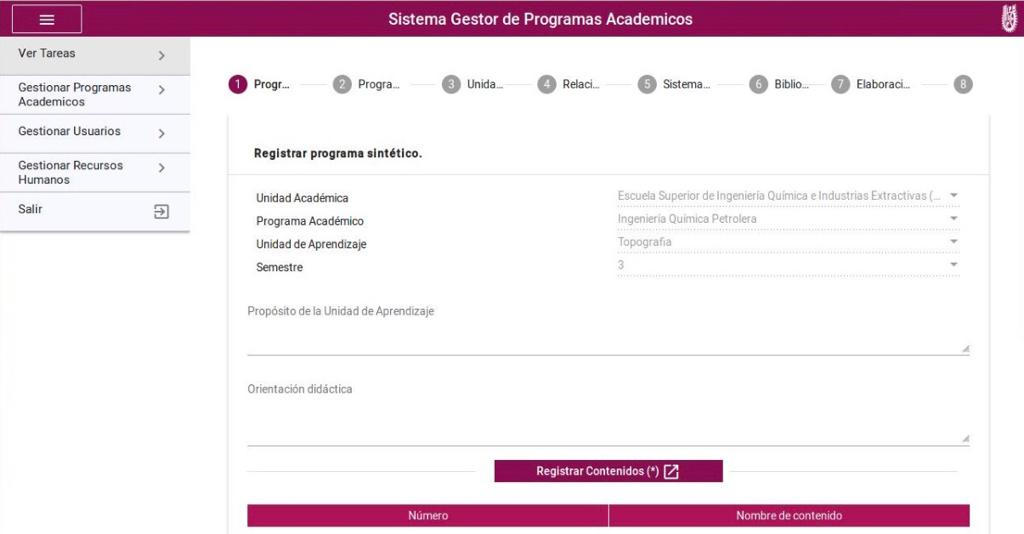
\includegraphics[width=0.7\linewidth]{images/SP6/PSinicio.jpeg}}
    
\includegraphics[width=0.7\linewidth]{images/SP6/PSinicio2.jpeg}
    \caption{Pantalla para Registrar Programa Sintético}
\end{figure}

Los campos desplegados en el formulario deberan ser llenados por el Docente.

Si el Docente desea:

\begin{itemize}
    \item Registrar Contenidos. El Docente deberá dar click sobre el botón \IUbutton{Registrar Contenidos(*)}. Posteriormente consulte \hyperlink{RegC}{Registrar Contenido}
    \item Registrar Evaluación y Acreditación. El Docente deberá dar click sobre el botón \IUbutton{Registrar Evaluación y Acreditación(*)}. Posteriormente consulte \hyperlink{RegEyA}{Registrar Evaluación y Acreditación}
\end{itemize}

Para concluir o guardar el previo registro checar:
\hyperlink{GuardarFinalizar}{Guadar y/o Finalizar}
\pagebreak
Si hay errores checar: \hyperlink{Errores}{Posibles Errores}
\pagebreak

\hypertarget{RegC}{\subsection{Registrar Contenido}}

Para registrar un Contenido correspondiente a un Programa Sintético, se debe acceder por medio del botón \IUbutton{Registrar Contenidos(*)} de la pantalla \hyperlink{RegistrarPS}{Registrar Programa Sintético}. Posteriormente se mostrará el siguiente formulario:

\begin{figure}[H]
    \centering
    \hypertarget{RegC}{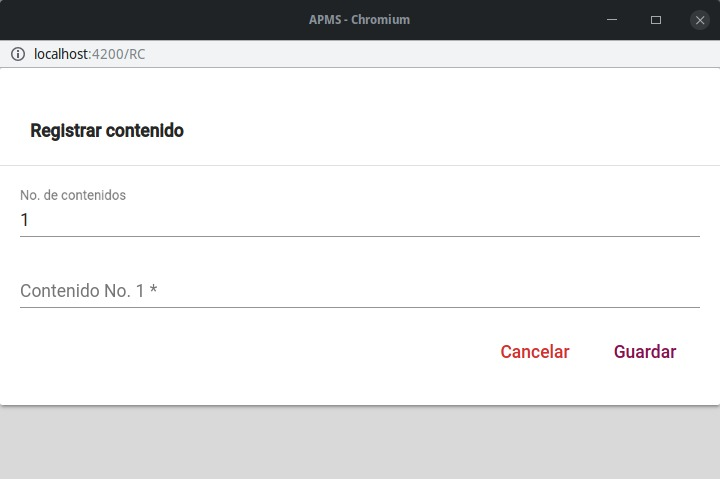
\includegraphics[width=0.5\linewidth]{images/SP6/11.jpeg}}
    \caption{Pantalla para Registrar Contenido}
\end{figure}
Para concluir el previo registro checar:
\hyperlink{AceptarCancelar}{Aceptar y/o Cancelar}

\pagebreak
\hypertarget{RegEyA}{\subsection{Registrar Evaluación y Acreditación}}


Para registrar la Evaluación y Acreditación correspondiente a un Programa Sintético, se debe acceder por medio del botón \IUbutton{Evaluación y Acreditación(*)} de la pantalla \hyperlink{RegistrarPS}{Registrar Programa Sintético}. Posteriormente se mostrará el siguiente formulario:


\begin{figure}[!h]
    \centering
    \hypertarget{RegEyA}{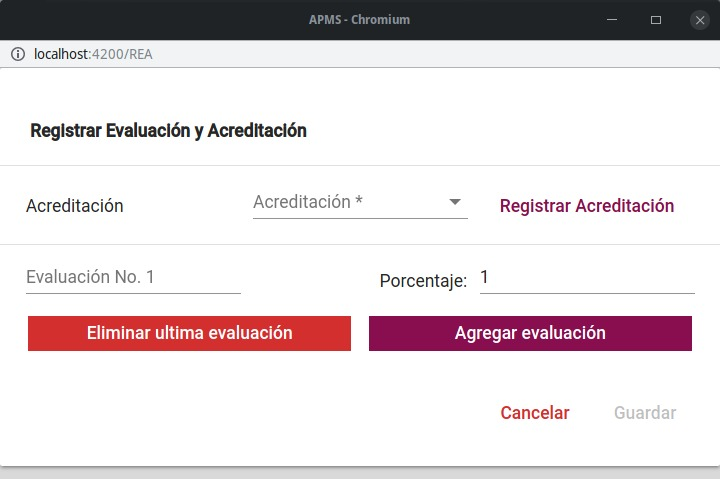
\includegraphics[width=0.5\linewidth]{images/SP6/8.jpeg}}
    \caption{Pantalla para Registrar Evaluación y Acreditación}
\end{figure}

Primeramente, el Docente deberá seleccionar el tipo de Acreditación. En caso de no estar registrado deberá dar click en el botón \IUbutton{Registrar Acreditación}(Consulte \hyperlink{RegA}{Registrar Acreditación}).

Posteriormente, se llenará el campo de evaluación con el nombre y el porcentaje asignado. De ser necesario un nuevo tipo de evaluación, el Docente deberá hacer click en el botón:

\begin{figure}[!h]
    \centering
    
\includegraphics[width=0.3\linewidth]{images/SP6/BotonEval.jpeg}
    \caption{Botón Agregar Evaluación}
\end{figure}

Y se desplegara un nuevo campo para el nombre de la evaluación y un nuevo campo para el procentaje de dicha evaluación.

Si el Docente desea eliminar la ultima evaluación agregada deberá dar click al botón:


\begin{figure}[!h]
    \centering
    
\includegraphics[width=0.3\linewidth]{images/SP6/BotonEliEval.jpeg}
    \caption{Botón Eliminar Evaluación}
\end{figure}
Para concluir el previo registro checar:
\hyperlink{AceptarCancelar}{Aceptar y/o Cancelar}
\pagebreak
\hypertarget{RegA}{\subsection{Registrar Acreditación}}

Para registrar un nuevo tipo Acreditación correspondiente a un Programa Sintético, se debe acceder por medio del botón \IUbutton{Registrar Acreditación} de la pantalla \hyperlink{RegEyA}{Registrar Evaluación y Acreditación}. Posteriormente se mostrará el siguiente formulario:


\begin{figure}[H]
    \centering
    \hypertarget{RegA}{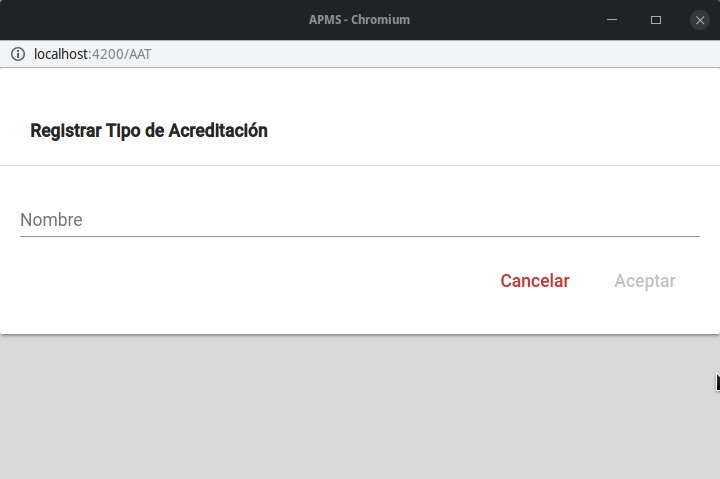
\includegraphics[width=0.5\linewidth]{images/SP6/9.jpeg}}
    \caption{Pantalla para Registrar Acreditación}
\end{figure}
Para concluir el previo registro checar:
\hyperlink{AceptarCancelar}{Aceptar y/o Cancelar}
\pagebreak